\section{Introduzione}

I programmi tradizionali elaborano l'informazione in modo radicalmente diverso
rispetto ai sistemi nervosi biologici. Un computer tradizionale è composto
sostanzialmente da un'unità di calcolo (processore, CPU), che esegue in
succesione un altissimo numero di operazioni; e da tre tipi di memoria: una che
contiene le istruzioni necessaria a svolgere le operazioni, una temporanea da
cui vengono letti i dati necessari e salvati i risultati dei calcoli effettuati
e una permanente in cui questi dati rimangono registrati. L'architettura e i
principi di funzionamento del computer seriale sono stati utilizzati dal
cognitivismo come metafora della mente; questa scelta presenta due vantaggi:
\begin{enumerate}
	\item \textbf{Formalismo}: la scienza dell'informazione fornisce un
	      formalismo scientifico e universalmente accettato con cui è possibile
	      descrivere il funzionamento della mente in modo univoco;

	\item \textbf{Modelli}: rende possibile l'impiego di modelli della mente
	      per la creazione di nuove tecnologie con caratteristiche di
	      intelligenza artificiale.
\end{enumerate}

Il sistema nervoso può essere paragonato a un'immensa società (Cervellopoli).
Ciascun abitante conosce quasi tutti gli abitanti del poprio paese o quartiere e
passa il proprio tempo a parlare con tutti loro.
Alcuni abitanti possiedono anche relazioni con individui che vivono in zone più
distanti e mantengono così la propria comunità continuamente aggiornata su
quello che succede.
La comunicazione è spesso caratterizzata da ripetizioni, rumore e
interruzioni.\\
L'elaborazione nei sistemi nervosi avviene in \textit{parallelo} (mentre nei calcolatori
tradizionali avviene in successione).
L'elaborazione nei sistemi nervosi è \textit{distribuita} su molti elementi.
Durante lo svolgimento dei compiti, si attivano molti neuroni, a volte
organizzati in gruppetti locali, altre volte distribuiti a macchie in zone
diverse nel cervello.
I sistemi nervosi non devono essere programmati per svolgere un compito, bensì
imparano autonomamente in base all'esperienza o con l'aiuto di un insegnante
esterno. Si ritiene che l'apprendimento consista soprattutto nella modifica
della "forza" delle connessioni attraverso cui i neuroni comunicano.

\subsection{Che cosa sono le Artificial Neural Networks (ANN)}

Le reti neurali artificiali sono dei sistemi di elaborazione dell'informazione,
il cui funzionamento trae ispirazione dai sistemi nervosi biologici. Una rete
neurale artificiale possiede molte semplici unità di elaborazione variamente
connesse tra di loro.
Alcune unità ricevono informazioni dall'ambiente (input),
altre emettono risposte nell'ambiente (output), altre ancora comunicano
solamente con le unità all'interno della rete (hidden).

\begin{figure}[H]
	\centering
	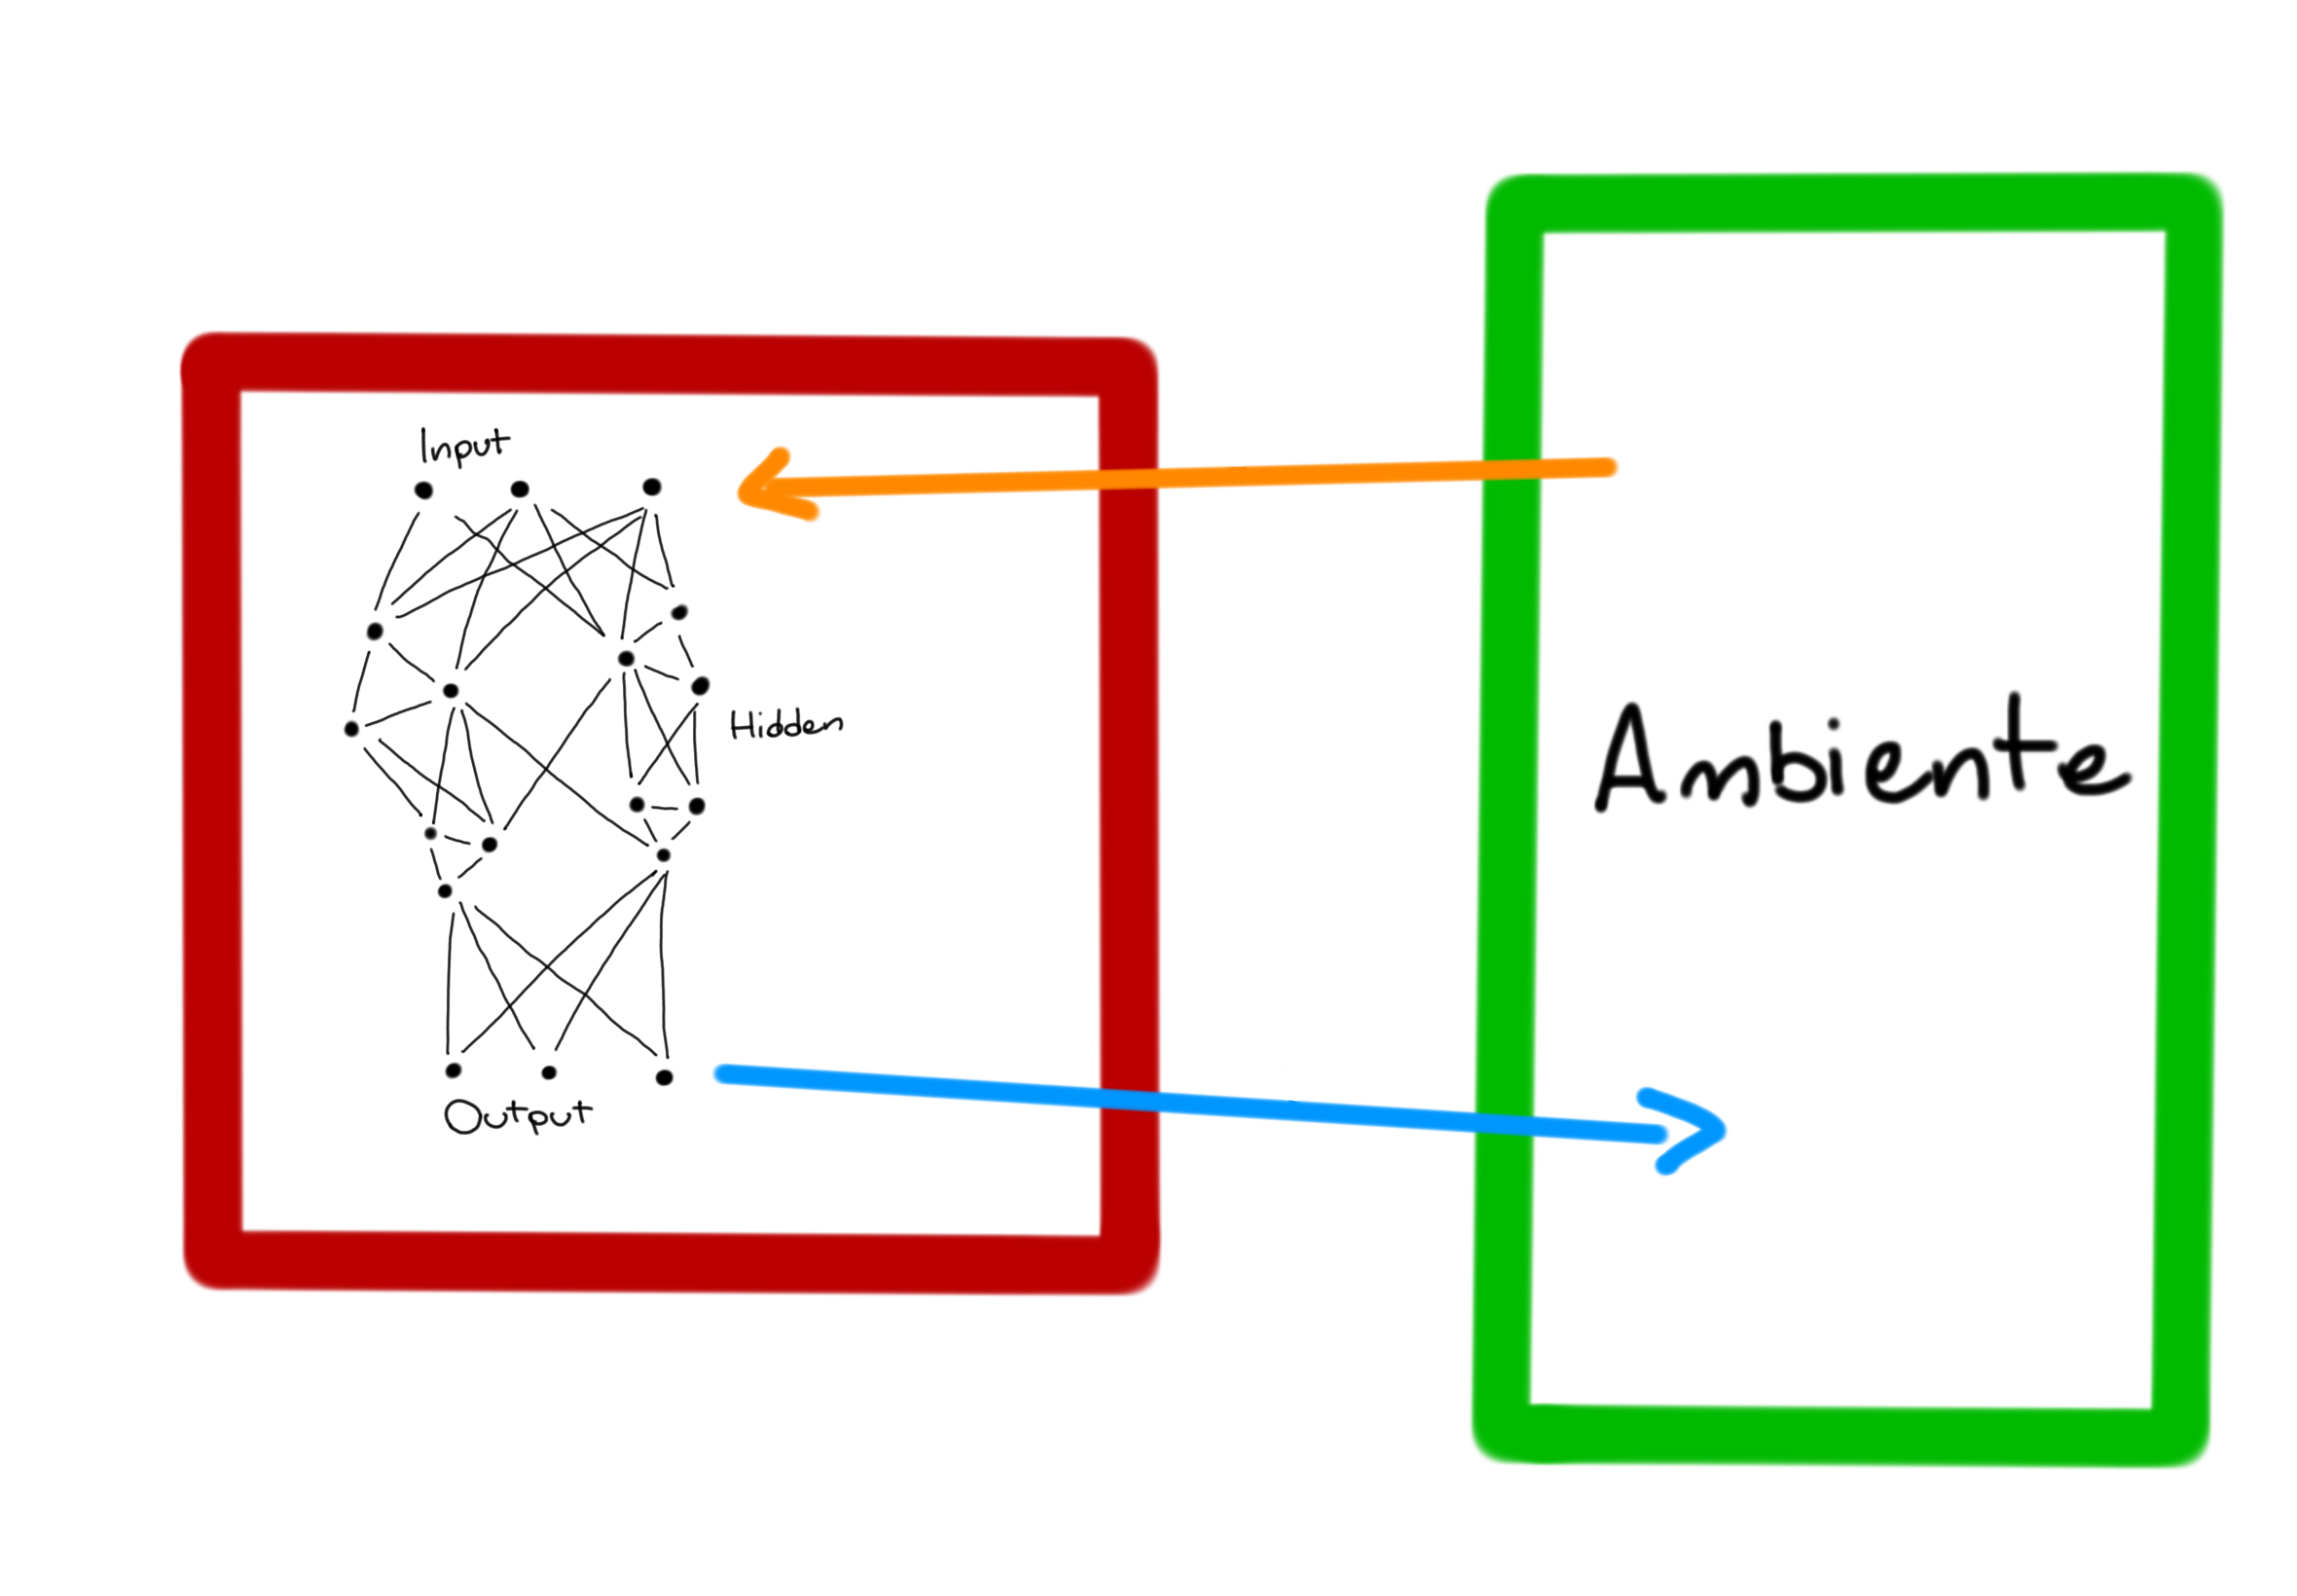
\includegraphics[width=0.7\textwidth]{ANN}
	\caption{Schema di una rete neurale artificiale}
\end{figure}

Ciascuna unità simula il ruolo di un neurone (infatti sono anche chiamate
neuroni o percettori (perceptrons)). Ciascuna unità diventa attiva se la
quantità totale di segnale che riceve supera la propria soglia di attivazione.
Ciascun punto di connessione agisce come un filtro che trasforma il messaggio
ricevuto in un segnale inibitorio o eccitatorio, aumentandone o diminuendone
l'intensità. Poiché il loro ruolo consiste in effetti nel pesare l'intensità dei
segnali trasmessi, essi vengono definiti anche con il nome di pesi sinaptici o
semplicemente pesi.

\begin{figure}[H]
	\centering
	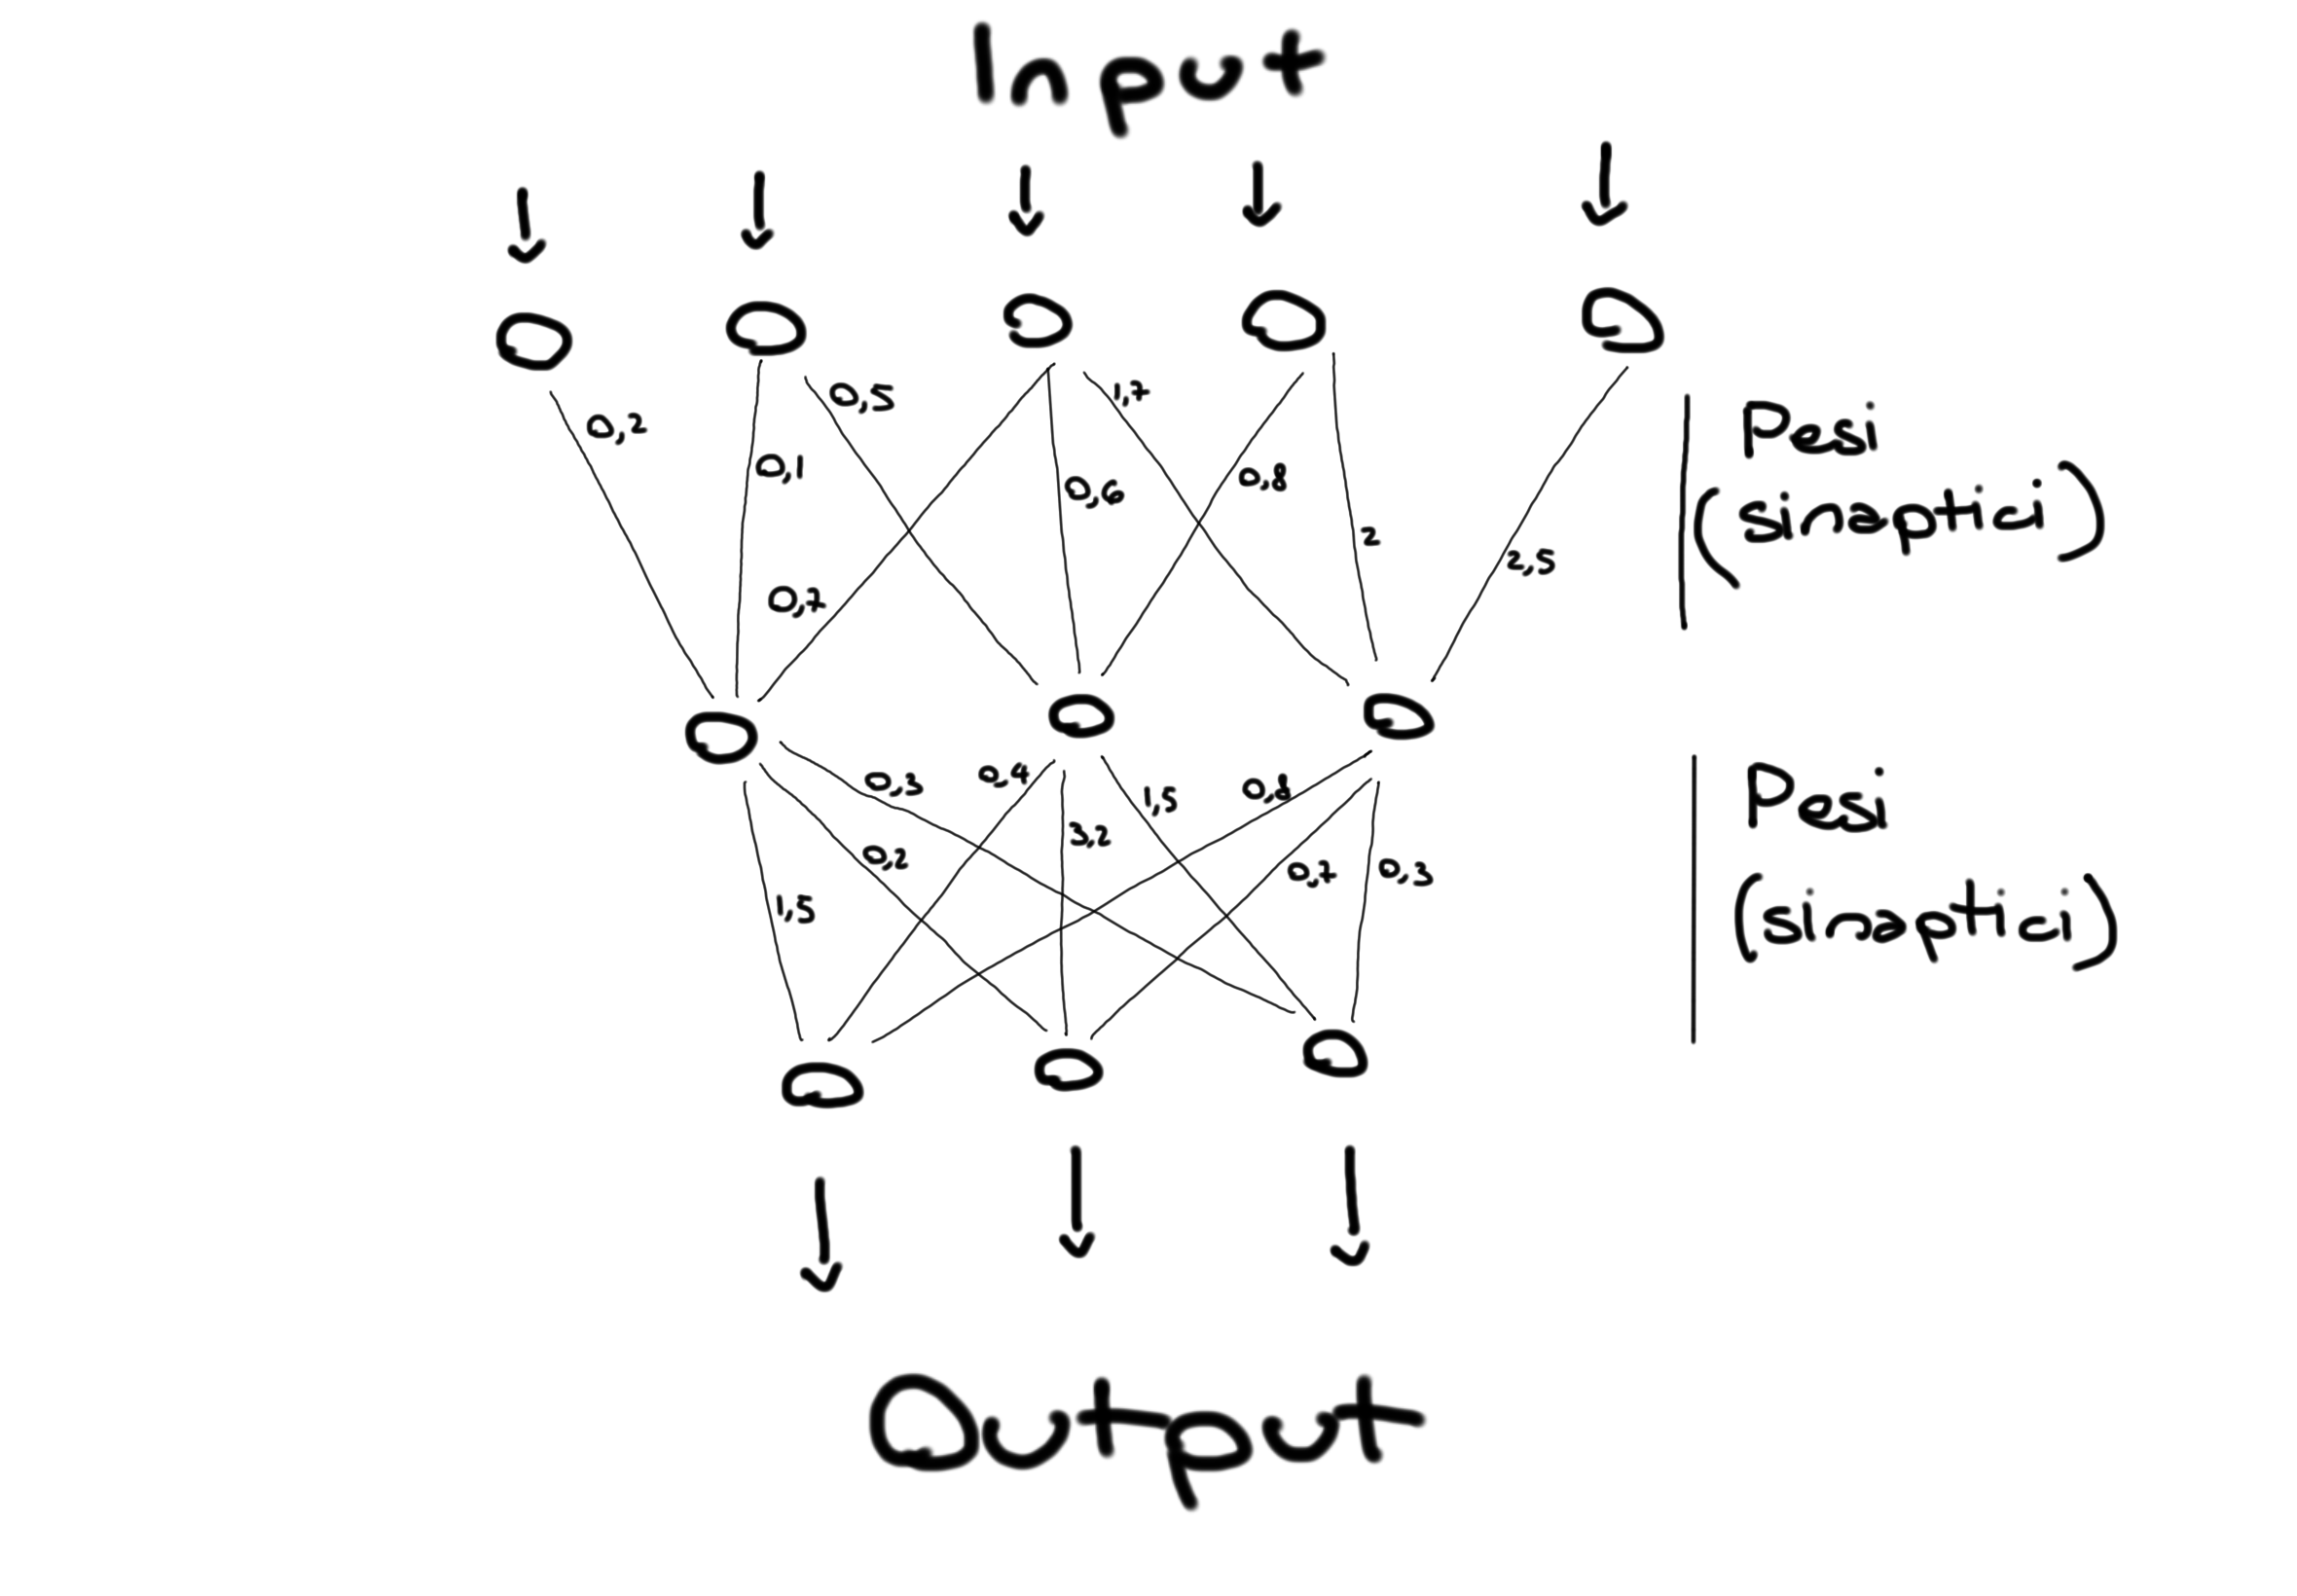
\includegraphics[width=0.7\textwidth]{Weights}
	\caption{Schema di una rete neurale artificiale}
\end{figure}

Formalmente, il segnale di risposta emesso da un nodo $n$, è uguale a
\begin{equation}
	n_i = \phi(\sum_{j \in \text{input}} w_{ij} \cdot n_j - \theta_i)
\end{equation}

Dove:
\begin{itemize}
	\item $n_j$ è l'output del nodo $j$;
	\item $w_{ij}$ è il peso della connessione tra $i$ e $j$;
	\item $\theta_i$ è la soglia di attivazione del nodo $i$;
	\item $\phi$ è una generica funzione di attivazione (ne studieremo alcune
	      all'interno del corso).
\end{itemize}

Quando uno stimolo viene applicato ai neuroni d'ingresso della rete neurale i
segnali viaggiano in parallelo lungo le connessioni attraverso i nodi interni
fino ai nodi di uscita la cui attivazione rappresenta la risposta della rete
neurale.
La configurazione delle connessioni e i valori delle sinapsi artificiali
determinano in gran parte il comportamento e la risposta della rete. Per questo
motivo si dice che le sinapsi rappresentano la conoscenza o memoria a lungo
termine della rete neurale. Nelle reti neurali la memoria è totalmente
distribuita e non richiede l'utilizzo di componenti aggiuntivi poichè è una
proprietà intrinseca del sistema stesso.\\
La regola di apprendimento di un modello neurale indica semplicemente le
condizioni locali e le modalità in cui le sinapsi si modificano a prescindere
dal tipo di compito per cui la rete verrà utilizzata.

\subsection{Caratteristiche delle ANN}

\begin{itemize}
	\item \textbf{Robustezza}: una ANN è resistente al rumore, ovvero è in grado
	      di continuare a dare una risposta corretta anche se alcune delle sue
	      connessioni vengono eliminate o se viene aggiunto del rumore al
	      segnale di ingresso;

	\item \textbf{Flessibilità}: una ANN può essere impiegata per un grande
	      numero di finalità diverse: non ha bisongo di conoscere le proprietà
	      del dominio specifico di applicazione perché le apprende in base
	      all'esperienza. Questa caratteristica rappresenta un vantaggio perché
	      permette di affrontare molti problemi di cui non sono note le
	      soluzioni analitiche. Tuttavia, si rischia di rinunciare a cercare di
	      comprendere a fondo la natura di un problema e di rifugiarsi in una
	      soluzione neurale che non aumenta la nostra conoscenza;

	\item \textbf{Generalizzazione}: una ANN allenata su un numero limitato di
	      esempi è in grado di produrre una risposta adeguata a dei pattern di
	      ingresso che non ha mai visto in precedenza, ma che presentano qualche
	      somiglianza con gli esempi presentati durante l'allenamento. In
	      effetti, una ANN estrae caratteristiche invarianti dei pattern di
	      ingresso piuttosto che memorizzare ciascun singolo pattern;

	\item \textbf{Recupero in base al contenuto}: le ANN sono in grado di
	      recuperare le proprie memorie in base al contenuto partendo da dati
	      incompleti, simili o corrotti da rumore.
\end{itemize}
